PanDA is a Workload Management System (WMS) designed to support the execution of
distributed workloads and workflows via pilots. WMS is middleware for
discovering and selecting resources, submitting tasks of workloads and
workflows, and monitoring their execution~\cite{marco2009glite}. Pilot is an
abstraction that enables multi-level scheduling by decoupling resource
acquisition from tasks scheduling~\cite{turilli2015comprehensive}. When
implemented, a pilot is scheduled on a site and, once active, tasks are
scheduled to the pilot, not to the site's scheduler.

Pilot-enabled WMS enable high throughput of tasks execution while supporting
interoperability across multiple sites. This is particularly relevant for LHC
experiments, where millions of tasks are executed across multiple sites every
month, analyzing and producing petabytes of data. The design of PanDA WMS
started in 2005 and its implementation went into production for the LHC Run 1 on
2009. PanDA was then extended with new subsystems to be deployed on Run 2, on
2015.

% We summarize PanDA's design, architecture, and execution process, focussing on
% those subsystems and components that are most relevant to the the integration
% of PanDA with supercomputers.

% \mtnote{TODO: replace `resource' with `site'; `http' to `HTTP'?}

% -----------------------------------------------------------------------------
\subsection{Design}
\label{ssec:panda_design}

PanDA's application model assumes tasks, workloads and workflows. Tasks
represent a set of operations performed on a set of events that are stored in
one or more input files. Tasks are decomposed into jobs, where each job
represents the task's set of operations and a partition of the task's events.
Since 2005, a certain amount of parallelism has been progressively introduced
for job execution~\cite{crooks2012multi} but, so far, no MPI jobs have been
considered for production. Jobs are supposed to be relatively self-contained,
capable of setting up their own execution environment or having a minimal set of
common dependences.

PanDA's usage model is based on multitenancy of resources and the support of at
least two types of HEP users: individual researchers and groups executing so
called `production' workflows. Users are free to submit tasks and workflows to
the PanDA WMS at any point in time, directly or via dedicated application
frameworks. Consistently, PanDA's security model is based on separation between
authentication, authorization and accounting for both single users and group of
users. Both authentication and authorization are based on digital certificates
and the X.509 standard and on the virtual organization (VO) abstraction.

Currently, PanDA's execution model is based on five main abstractions: task,
job, queue, pilot, and event. Both tasks and jobs are assumed to have attributes
and states and to be queued into a global queue for execution. Prioritization
and binding of jobs are assumed to depend on the attributes of each job. Pilot
is used to indicate the abstraction of resource capabilities. Each job is
thought to be bound to one pilot and executed on the site where the pilot has
been instantiated.

In PanDA's data model, each event refers to the recorded or simulated
measurement of a physical event. One or more events can be packaged into files
or other data containers. As with jobs, data have both attributes and states,
and some of the attributes are shared between events and jobs. Raw,
reconstruction, and simulation data are assumed to be distributed across
multiple storage facilities and managed by the ATLAS Distributed Data Management
(DDM)~\cite{garonne2012atlas}. When necessary, datasets required by each job are
assumed to be replicated over the network, both for input and output data.

PanDA's design supports provenance and traceability for both jobs and data.
Attributes enable provenance by linking jobs and data items, providing
information like ownership or project affiliation. States enable traceability by
providing information about the stage of the execution in which each job or data
item is or has been. Some attributes are assumed to be immutable across
execution and jobs and data items are assumed to be always in one and only one
state.


% \begin{itemize}
%   \item No MPI tasks?
%   \item Pilot multitenancy?
%   \item PanDA Server Brokerage component and Event service interaction?
%   \item PanDA Server Data Service component and Event Service interaction?
% \end{itemize}

% Different types of job payload (i.e., executable) are assumed, both in terms
% of user-defined batch scripts or application frameworks for group of users.

% Consistently, pilots are considered to be multitenant as jobs belonging to
% multiple workflows and/or users can be bound and executed on them.
% PanDA' data model mostly uses events as the unit of data
% \mtnote{Is event an abstraction specific to the MD workflow?}.

% \sergeynote{Raw data from the ATLAS detector is captured at CERN and goes
% through reconstruction step to produce data in secondary formats, smaller in
% volume and with more and more physics content instead of raw detector hits.
% Consequently a second, custodial, copy of raw data is being distributed in
% predetermined volumes to National T1 centers around the world (like BNL  T1
% center). This insures low raw data redundancy and safety. Multiple copies of
% chunks of secondary data sets (derived from real raw data) are also
% distributed to ~100 centers around the word for ease of access and improved
% availability for analysis. Then raw detector data is stored on Tapes at CERN,
% just  in case. Most users, who do physics analysis, rarely work with raw
% data, only a small group of experts needs to work with raw data for
% specialized tasks like detector calibrations and such. There may be a need to
% redo a reconstruction step, when errors in previous reconstruction campaign
% are uncovered or improved detector understanding will lead for a better
% quality physics. Then data stored on tape is recovered and re-processed
% again. Simulation data is produced in many places anyway and is not
% centralized to begin with. Here's the paper that describes current DDM state
% in ATLAS, data replication strategies and such.
% http://iopscience.iop.org/article/10.1088/1742-6596/396/3/032045/pdf DDM is a
% complex and evolving topic in ATLAS.}\mtnote{Thank you. As we are describing
% the design of PanDA I thought we should not enter into a too detailed
% description of the DDM design. I eliminated the mistake I had made about
% `centralized data' but left DDM just as a reference. Any better?}


% -----------------------------------------------------------------------------
\subsection{Implementation and Execution}
\label{ssec:panda_arch}

\mtnote{From Danila: DDM enacts decisions about registering files into datasets.
These decisions are made by productions. DDM DOES OT DECIDE which file should be
in which dataset.}\mtnote{Done.}
\mtnote{No communication between APF and PanDA Server (deleted arrow, adjust
numbers and related text)}\mtnote{Done.}
\mtnote{No more DDM Service on Edge on grid sites. DDM directly interacts with
SE (deleted arrows, moved number 8. Update labels and related text)}\mtnote{Done.}

The implementation of PanDA consists of several interconnected subsystems, most
of them built from off-the-shelf and Open Source components. Subsystems
communicate via dedicated API or HTTP messaging, and each subsystem is
implemented by one or more modules. Databases are used to store eventful
entities like tasks, jobs and events, and to store information about sites,
resources, logs, and accounting.

Currently, PanDA's architecture has five main subsystems: PanDA
Server~\cite{maeno2011overview},
AutoPyFactory~\cite{caballero2012autopyfactory}, PanDA
Pilot~\cite{nilsson2011atlas}, JEDI~\cite{borodin2015scaling}, and PanDA
Monitoring~\cite{klimentov2011atlas}. Other subsystems are used by some of ATLAS
workflows (e.g., PanDA Event Service~\cite{calafiura2015atlas}) but, at the
moment, they are not relevant to understand how PanDA has been ported to
supercomputers. For a full list of subsystems see Ref.~\cite{panda-wiki_url}.
Figure~\ref{fig:architecture} shows a diagrammatic representation of PanDA main
subsystems, highlighting the execution process of tasks while omitting
monitoring details to improve readability.

\begin{figure}
  \begin{center}
    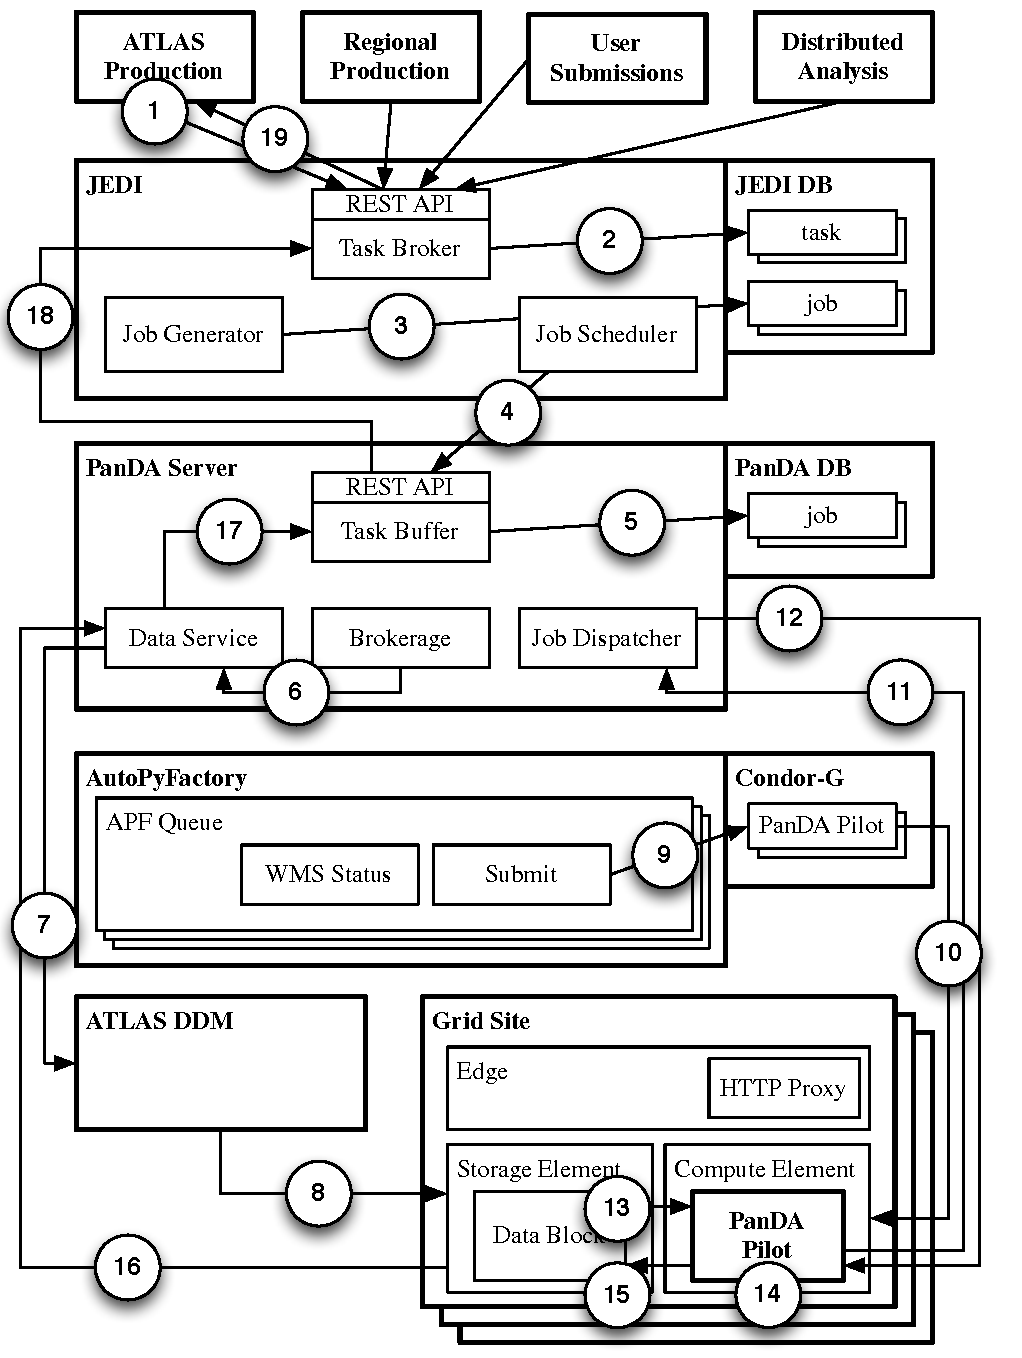
\includegraphics[width=\columnwidth]{figures/panda_architecture.pdf}
  \end{center}
    \caption{PanDA architecture with the subsystems and components
    relevant to the integration of PanDA with supercomputers. Numbers indicates
    the execution process based on JEDI: From the submission of tasks (1) to the
    retrieval of their output (19). The monitoring subsystem, the architectural
    details of PanDA Pilot and the communication among subsystem's components
    are abstracted to improve clarity.}
\label{fig:architecture}
\end{figure}

% -----------------------------------------------------------------------------
% PANDA SERVER
% -----------------------------------------------------------------------------
% \textbf{PanDA Server} is the central hub service of PanDA WMS and it operates
% as a web service~\cite{maeno2011overview}. It consists of four main components
% implemented in Python: Task Buffer, Brokerage, Job Dispatcher, and Data
% Service. Together, these components implement a global queue where to store
% jobs, share information about jobs and their dataset properties with the other
% subsystems, and update their states at execution time.
% -----------------------------------------------------------------------------

% It runs on Apache web server, interacting with the back-end database running
% on separate machines. PanDA Server implements the Apache worker model, with
% many independent processes handling client requests in parallel. Since all
% state is maintained in the central database, the PanDA Server instance itself
% is stateless. Currently, the production version of PanDA utilizes an Oracle
% database as backend, but PanDA Server can also work with the MySQL family of
% databases.

% . It provides a task queue
% managing all job information centrally. The PanDA server receives jobs through
% the client interface into the task queue, upon which a brokerage module
% operates to prioritize and assign work on the basis of job type, priority,
% input data and its locality, and available CPU resources. The PanDA server
%
% and communicating via Python APIs

% Task Buffer manages PanDA's global queue by: (i) storing jobs into the global
% queue; (ii) providing information about and updating the state of each stored
% job. The Brokerage component: (i) matches job attributes with site and pilot
% attributes; (ii) manages the dispatch of input data to processing sites; and
% (iii) derives PanDA's data pre-placement requirement. The Job Dispatcher: (i)
% receives requests from active pilots for new jobs to process; (ii) retrieves
% from Task Buffer the jobs with highest priority and that can be executed on
% the site of the requesting pilot; (iii) creates a wrapper script for the
% selected job, tailored to the site of the requesting pilot; and (iv) monitors
% the state of the job execution on the pilot, updating the Task Buffer
% component. Finally, the Data Service component: (i) retrieves information from
% Task Buffer and Brokerage about the data requirements of each job and the site
% to which each job has been assigned; (ii) interacts with the ATLAS DDM to make
% input files available to the jobs and manage their output data.

% -----------------------------------------------------------------------------
% PANDA PILOT
% -----------------------------------------------------------------------------
% \textbf{PanDA Pilot} implements the execution environment for PanDA's
% jobs\cite{nilsson2011atlas}. Implemented in Python, a PanDA Pilot is launched
% by a wrapper script submitted to a site. Wrapper scripts are tailored to the
% middleware exposed by each site so to maintain PanDA Pilot site-independent.
% PanDA Pilot pulls a job for execution, sets up the execution environment
% including the required input files, spawns the jobs's executable, monitors its
% execution, and supports the output's staging.
% -----------------------------------------------------------------------------

% t: (i) prepares the execution environment for PanDA's jobs, collecting
% information about the compute, data, and network capabilities of the site;
% (ii) requests a job for execution to the Job Dispatcher component of PanDA
% Server; (iii) initiates and monitors the execution of pulled jobs, including
% setting up the job, transferring its input when required, executing the
% payload, transferring output, and checking log files and local space; and (iv)
% cleans up when the payload has finished to execute.

% PanDA is a pilot based workload management system.
% In the PanDA job lifecycle, pilot jobs (Python scripts that organize workload
% processing on a worker node) are submitted to sites. When these pilot jobs
% start on a worker node they contact a central server to retrieve a real
% payload (i.e., an end-user job) and execute it.

% -----------------------------------------------------------------------------
% PILOT DESCRIPTION: COMMENTED OUT BECAUSE WE DESCRIBE IT LATER ON.
% -----------------------------------------------------------------------------
% PanDA Pilot implements the pilot paradigm~\cite{turilli2015comprehensive},
% decoupling resource acquisition from job execution via multi-stage scheduling.
% This has several benefits, including increasing throughput by lowering the
% time taken to queue and schedule jobs; enabling both concurrent and
% sequential job execution depending on the number of cores available to the
% pilot and the time for which it remains available; and exposing a unified and
% consistent interface for the scheduling of jobs, independent from the
% middleware of the site on which the pilot has been instantiated.
% -----------------------------------------------------------------------------

% The specific implementation of PanDA Pilot promotes reliability by
% monitoring the execution of the job's payload, and a certain degree of
% fault-tolerance by recovering information and, possibly, output files from
% jobs that failed, even before instantiating the PanDA Pilot.

% Using these pilot-based workflows helps to improve job reliability, optimize
% resource utilization, allows for opportunistic resources usage, and mitigates
% many of the problems associated with the inhomogeneities found on the Grid.

% Upon bootstrapping, PanDA Pilot downloads major parts of its runtime code via
% HTTP from a central Subversion repository. The repository works with an Apache
% web server, configured with a memory-based web proxy (Squid). The purpose of
% the cache is to reduce the request load on the back-end Subversion server.
% That improves performance since only occasional queries trigger a full lookup
% on the back-end Subversion system, and most external queries are pulled from
% memory on the front-end web server. The benefits of this system include a
% high-performance code download service, combined with code updates still being
% immediately available as soon as they are committed to source code control.

% -----------------------------------------------------------------------------
% AUTOPYFACTORY
% -----------------------------------------------------------------------------
% \textbf{AutoPyFactory} implements a factory to submit pilots locally and to
% both grid and cloud sites~\cite{caballero2012autopyfactory}. Implemented to be
% executed as a single demonized process, AutoPyFactory concurrently spawns
% multiple processes called APFQueue that, on the base of information about jobs
% queued on the PanDA server and on the state and capabilities of resources,
% submit pilots to multiple sites with Condor-G~\cite{frey2002condor}.
% -----------------------------------------------------------------------------

% Each APFQueue communicates with PanDA Server and the Brokerage module to
% collect information about the state of the jobs it manages. On the basis of
% this information, an APFQueue submits new pilots to one site. AutoPyFactory
% implements functionalities to evaluate the number of pilots already
% instantiated on each site, and to apply a consistent and adequate pressure on
% their batch queues. Submission is performed via the Condor-G batch
% system~\cite{frey2002condor}, enabling submission to multiple type of sites.
% AutoPyFactory exposes a dedicated monitoring service, feeding information to
% the PanDA Monitoring subsystem. A proxy manager enables certificate-based
% authentication and authorization for each site.

% As a pilot-based system, PanDA requires some way to get the initial PanDA
% pilot onto worker nodes at sites. This is done with the help of a component
% called AutoPyFactory (APF). APF runs in a single daemonized process,
% launching a separate thread for each internal workflow. Each one of these
% internal workflows typically serves a single job queue as defined in WMS, and
% delivers pilots to a single batch queue, either local or remote. The behavior
% of these APF workflows is determined by the combination of a set of plugins,
% invoked in a fixed order, in a loop, each one in charge of the performance of
% a well defined action.

% -----------------------------------------------------------------------------
% PANDA MONITORING - SPACE SAVING
% -----------------------------------------------------------------------------
% \paragraph{\textbf{PanDA Monitoring}} this subsystem is implemented as a
% web-based, dashboard-style graphical application~\cite{klimentov2011atlas}. It
% runs on Apache and interacts with the back-end database of PanDA Server to
% enable persistence. PanDA Monitoring enables users and site administrators to
% gather information about the status of current and past jobs, data movement,
% and pilot factory. PanDA Monitoring allows users access to all log files of
% each job, greatly simplifying code debugging and failure analysis in a
% distributed computing environment.
% -----------------------------------------------------------------------------

% -----------------------------------------------------------------------------
% JEDI
% -----------------------------------------------------------------------------
% \textbf{JEDI} exposes a task abstraction for workload and workflows
% specification and interfaces with PanDA Server to manage their execution on
% remote sites~\cite{borodin2015scaling}. Implemented as a standalone service,
% JEDI partitions tasks to jobs, and binds these jobs to sites via dedicated
% queues. JEDI collects information about sites' resource capability,
% availability, and performance. Based on this information, JEDI associates
% sites with similar capabilities to a queue. JEDI replaces and extends the
% Brokerage module of the PanDA Server.
% -----------------------------------------------------------------------------

% Each job is assigned to a queue by matching the job's requirements to the
% capability, availability and performance of the sites of that queue. In this
% way,

% This module still handles communication between the Task
% Buffer and the Data Service modules.


% -----------------------------------------------------------------------------
% \subsection{Execution}
% \label{ssec:panda_exec}

% The tasks of workloads and workflows submitted to PanDA are partitioned
% to one or more jobs. Each job is then executed on one of the available
% PanDA Pilots, chosen among those that the PanDA Server manages across multiple
% sites. Tasks processes a certain amount of events that are stored into files,
% and when a task is partitioned to multiple jobs, subsets of events need to be
% assigned to each job and made available to the pilot on which that job will be
% executed. Finally, the output of each job need to be retrieved and aggregated
% into the output of the original task (Fig.~\ref{fig:architecture}).

The relation between tasks and jobs can be one-to-one or one-to-many, and the
conversion between the two can by static or dynamic. During the LHC Run 1, PanDA
required users or applications to perform a static conversion between tasks and
jobs: tasks were described as a set of jobs
% with a fixed number of events
and then submitted to the PanDA Server.

This approach introduced inefficiency both with usability and resource
utilization~\cite{borodin2015unified}. Ideally, users should not have to reason
in terms of jobs: Users conceive analyses in terms of one or more, possibly
related tasks; the `job' abstraction is required by the execution middleware,
i.e. PanDA. Further, a static partitioning of tasks into jobs does not take into
account the heterogeneity and dynamicity of the resources of the pilots on which
each job will be executed.

Another problem of static job sizing is that PanDA instantiates pilots on sites
with different type of resources and different models of availability of those
resources. An optimal sizing of each job should take into account these
properties. For example, sites may offer cores with different speed, networking
with different amount of bandwidth, and resources could be guaranteed to be
available for a defined amount of time or could disappear at any point in time
as with opportunistic models of resource provision.

JEDI was deployed for the LHC Run 2 to address these inefficiencies. Users or
the application layer submits tasks descriptions to JEDI
(Fig.~\ref{fig:architecture}:1) that stores them into a queue implemented by a
database (Fig.~\ref{fig:architecture}:2). Tasks are partitioned into jobs of
different size, depending on both static and dynamic information about available
resources (Fig.~\ref{fig:architecture}:3). Jobs are bound to sites with
resources that best match jobs' requirements, and submitted to the PanDA Server
for execution (Fig.~\ref{fig:architecture}:4).

Once submitted to the PanDA Server, jobs are stored by the Task Buffer component
into a global queue implemented as a  database (Fig.~\ref{fig:architecture}:5).
When jobs are submitted directly to the PanDA Server, the Brokerage component is
used to bind jobs to available sites, depending on static information about the
resources available for each site. Jobs submitted by JEDI are already bound to
sites so no further brokerage is needed.

Once jobs are bound to sites, the Brokerage module communicates to the Data
Service module what data sets need to be made available on what site
(Fig.~\ref{fig:architecture}:6). The Data Service communicates these
requirements to the ATLAS DDM (Fig.~\ref{fig:architecture}:7) that, when needed,
takes care of % aggregating files into datasets and containers,
replicating them on the required sites (Fig.~\ref{fig:architecture}:8).

% AutoPyFactory subsystem communicates with the Task Buffer component of the
% PanDA Server, acquiring information about jobs that are ready for execution on
% specific (type of) sites (Fig.~\ref{fig:architecture}:9). On the basis of this
% information,
Meanwhile, AutoPyFactory defines a set of suitable PanDA Pilots and concurrently
submits them to a Condor-G broker (Fig.~\ref{fig:architecture}:9). This broker
submits these pilots wrapped as jobs or VMs to the required sites
(Fig.~\ref{fig:architecture}:10).

% AutoPyFactory submits pilots only when similar pilots are not yet available
% and maintains a predefined amount of pressure on the queue of each site. In
% this way, resource availability and utilizations is optimized.

When a PanDA Pilot becomes available on a site, it calls the Job Dispatcher
module of the PanDA Server, requesting for a job to execute
(Fig.~\ref{fig:architecture}:11). The Job Dispatcher interrogates the Task
Buffer module for a job that is bound to the site of that pilot and ready to be
executed. Task Buffer checks the global queue (i.e., the PanDA database) and,
upon availability, returns a suitable job the Job Dispatcher. The Job Dispatcher
dispatches that job to the PanDA Pilot (Fig.~\ref{fig:architecture}:12).

% \mtnote{Can a pilot request multiple jobs to execute
% concurrently?}\sergeynote{In principle it should be able to do that, but
% that's not how it is operated. One pilot - one job is a cleaner model in an
% environment where resources are ``owned'' by the organization that runs
% pilots. Simplifies many things. At least as far as I know.}

Upon receiving a job, a PanDA Pilot starts a monitoring process and forks a
subprocess for the execution of the job's payload. The job is set up, input data
are transferred from the designated staging-in location
(Fig.~\ref{fig:architecture}:13), and the job's payload is executed
(Fig.~\ref{fig:architecture}:14). Once completed, output is transferred to the
staging-out location (Fig.~\ref{fig:architecture}:15).

% During the job's payload execution, the monitoring process of PanDA Pilot
% checks the status of the job execution and its environment.

The Data Service module of the PanDA Server tracks and collects the output
generated by each job (Fig.~\ref{fig:architecture}:16), updating jobs'
attributes via the Task Buffer module (Fig.~\ref{fig:architecture}:17). When the
output of all the jobs of a task are retrieved, it is made available to the user
via PanDA Server. When a task is submitted to JEDI, task is instead marked as
done (Fig.~\ref{fig:architecture}:18) and the result of its execution is made
available to the user by JEDI (Fig.~\ref{fig:architecture}:19).

% \mtnote{Think whether a comparison with other WMS based on the review we did
% makes sense in this context.}\sergeynote{You provided a nice description of
% the PanDA system here.}
